\documentclass{report}

\usepackage{framed}
\usepackage{alltt}
\usepackage{graphicx}

\begin{document}
\title{Technical Report}
\author{Lu\'{\i}s Pureza}

\maketitle

\tableofcontents

\addtolength{\parskip}{\baselineskip}

\chapter{The prototype}

My goal is to develop a stand-alone interpreter that receives the name
of an EzQL file in the command-line, as well as some configuration for
the input adapters, and executes the code as events arrive in those
adapters. For example:

\begin{verbatim}
$ ./ezql linear-road.ezql PosSegStr=file://pos-seg-stream.csv
\end{verbatim}

This would execute the linear-road.ezql file, using the file
pos-seg-strem.csv as input to the \verb=PosSegStr= stream. Below we
show some possible contents of this file:

\begin{verbatim}
timestamp, vehicleId, speed, segNo, dir, hwy
        0,        10,    50,     3,   1,   3
      100,         5,    40,     6,   0,   2
      130,         2,    35,     2,   1,   1
\end{verbatim}

Each line (except the first) represents an event that will be fed up
to the \verb=PosSegStr= stream at the given timestamps. In this
example, the first event will be sent to the stream as soon as the
application is ready, the second will follow 100 milliseconds later,
the third 130 milliseconds later and so on.

Naturally, this approach is good for testing and validation, but the
real world doesn't work this way -- we don't know the events
beforehand! One could implement some other kind of input adapter (for
example, one which receives events from some network socket), but this
issue is orthogonal to this internship.

Why a stand-alone interpreter and not an application-server? Well,
because it seems to be the fastest and easiest route to have something
that works. I see no reasons why an application-server that executes
EzQL applications could not be written in the future.

And finally, why an interpreter and not a full-blown compiler? Again,
fastest route. A compiler would take considerable time to write and
test, and if I was to implement one during this internship, the EzQL
language would necessarily have less features. I prefer to prove that
the language can do many things well compared to what's in the state
of the art. Optimization comes later, if this is ever going to be used
in production.


\chapter{Execution model}

EzQL supports two modes of execution: continuous and ``one-shot''. The
first is what we usually call ``continuous queries'', i.e., ``queries
that are issued once and then logically run continuously over the
database (in contrast to traditional one-time queries which are run
once to completion over the current data sets)'' (taken from
``Continuous Queries over Data Streams'', by Babu and Widom).

Take, for instance, the following program:

\begin{verbatim}
stocks = Stream of { :symbol, :price }

@createFrom(stocks, :symbol)
class Company
end

cheap_companies =
  from c in all Company
  where c.price < 10
  select c
\end{verbatim}

\verb=cheap_companies= is a collection that contains -- \emph{at any
  moment} --, the companies whose stocks are worth less than \$10. The
query that generates this collection is \emph{active} while the
program is running. As soon as a new price report is received, the
query will be executed and the corresponding company object may be
added or removed from \verb=cheap_companies=. This is completely
transparent to the developer, because he doesn't need to specify when
this computation should take place. The engine takes care of the
details. All the developer needs to know is that the contents of that
collection are always consistent with what the user expects them to
be. In a way, I would consider this an abstraction.

There are situations when one wants to execute some action in a
one-shot way. These actions could be scheduled in advance -- ``Print
the symbols of all the cheap\_companies at 11:00 am'' --, or could
happen in response to some event -- ``when the car moves to a new
segment, calculate the new toll for that segment''. In my opinion,
these actions are mostly useful for their side-effects and continuous
queries are not appropriate to handle them. The following query, taken
from the linear road benchmark solution in CQL, shows this:


\begin{verbatim}
Select Rstream(E.vehicleId,
               basetoll * (V.numVehicles - 150)
                        * (V.numVehicles - 150) as toll)
From VehicleSegEntryStr [Now] as E,
     CongestedSegRel as C, SegVolRel as V
Where E.segNo = C.segNo and C.segNo = V.segNo and
      E.dir = C.dir and C.dir = V.dir and
      E.hwy = C.hwy and C.hwy = V.hwy
\end{verbatim}

According to the semantics of CQL, this query is executed when a
vehicle switches segments (an event that goes into
\verb=VehicleSegEntryStr[Now]=). But what happens when a previously
congested segment stops being congested? Or when the number of
vehicles in a segment changes? Well, as long as no vehicles switch
segments, the join condition will fail and nothing will be produced. I
find it hard to reason about the runtime behavior of programs this
way. It gets more complicated when we join several windows
together. Should a new result be produced every time one of the
windows change? Is this what the user wants? I'd rather have the
option to express these actions using something along the lines of:

\begin{verbatim}
when <vehicle v switches to segment s>
    s.updateToll()

...

class Segment
    ...

    def updateToll()
        if this.isCongested then
            this.toll = basetoll * (this.vehicles.length - 150) ^ 2
    end

\end{verbatim}

This snippet should be easily understandable, except maybe how to
determine that a segment is congested, and how to find out the
\verb=Segment= object corresponding to the segment the vehicle just
entered. I'll ignore these details for now.

The important thing to retain is that everything inside the
\verb=when= (including the call to the \verb=updateToll()= method) is
executed sequentially, just like a Java or Python program.

Naturally, \verb=toll= is an attribute of any segment that may be used
in queries:

\begin{verbatim}
cheap_tolls =
  from s in all Segment
  where s.toll < 10
  select s
\end{verbatim}

One thing I haven't decided yet is if we should allow queries inside
pieces of code that are going to be executed sequentially. For
example:

\begin{verbatim}
when <vehicle v switches to segment s1>
    <calculate and print the average speed in that segment over
     the last 5 minutes>
\end{verbatim}

This is a one-time query that runs until completion every time a
vehicle switches to a specific segment. As it is not a continuous
query, the system must be aware that it needs to save the last 5
minutes of data for that segment. What about the other segments?
Should it keep their data too, or is it smart enough to figure out, by
looking at the code, that only segment s1 will be necessary?

\chapter{Language paradigm}
The way I see it, the paradigm is event-driven with a topping of
procedural, declarative and OOP programming.

In EzQL you say what to do when an event arrives and that's it. If
there are no events, nothing is executed. There is no \verb=main= and
no global \verb=while(true)=. Of course, you can have dummy events
created by the system so that the application has something to do even
when there are no external events.

Another big difference is that code is not executed in a sequential
way. When an event arrives, a set of queries may be triggered into
execution, but these do not need to be declared next to each other in
the source code. The only place where the execution is guaranteed to
be sequential is inside \verb=when= blocks and functions (more on this
below).

I believe that having continuous queries and \verb=when= blocks should
be enough to handle most problems in a practical
way\footnote{Actually, I'm still skeptic, but I'm yet to see a problem
  that can't be easily solved using these constructs.}.

You may define and use functions and classes. The following sections
discuss this.

\section{Procedural programming in EzQL}

EzQL supports functions just like other programming languages, but
with a few rules. First, you cannot call a function from the top-level
(i.e., \verb=main()= in Java). Actually, there doesn't even exist a
top-level in EzQL. To see why, consider the following code:

\begin{verbatim}
def f()
    print "Hello world"
end

class Segment
end

f()   # <<<<<<<<<<<<<<<<<<<<<<

cheap_tolls =
  from s in all Segment
  where s.toll < 10
  select s
\end{verbatim}

When should \verb=f= be called? During start-up? Every time an event
arrives? The former makes some sense, but we may as well create some
kind of ``initialization area'' and stick it there:

\begin{verbatim}
when Initializing # Initializing is a dummy event
    f()
\end{verbatim}

This may seem a \verb=main()= method in disguise. Note, however, that
when \verb=f= returns and the \verb=when= block terminates, the
program remains in execution.

You may call functions from anywhere inside a \verb=when= block, or
from other functions. This is just like regular sequential programming
and should be clear.

You may also call functions from specific points in continuous
queries, in particular, inside \verb=where= filters and \verb=select=
statements:

\begin{verbatim}
def lessThan(value, threshold)
    value < threshold
end

def log(value)
    ...
end

cheap_tolls =
  from s in all Segment
  where lessThan(s.toll, 10)
  select log(s.toll)
\end{verbatim}

I would also like to allow the user to implement his own aggregates
and even operators (i.e., his own \verb=where=, \verb=select=, etc)
because there's no way the standard ones will be enough. This is very
low priority stuff though and would require much more time than I
possess (besides, it is difficult to convince people that the standard
operators are not enough).

\section{Classes}

In EzQL, classes are used to model entities. It is not clear, at this
point, if we should allow the developer to use classes for other
things like creating a \verb=LinkedList= class. Also, at this point,
inheritance is not supported. Should it be?

The attributes of an object are, by default, continuous values, which
is another way to say that they follow the state-changes
semantics. However, sometimes we need the pulse sematics. For example:


\begin{verbatim}
stocks = Stream of { :symbol, :price, :volume } # Volume is new here

@createFrom(stocks, :symbol)
class Company
end

from c in all Company
where c.volume > 1000
\end{verbatim}

This is wrong because volume is undefined between events. It's just
like the noise level in a street between sensor readings: there was a
value, but the system doesn't know it. It may have been quiet or an
ambulance may have passed. We don't know anything, so the only
sensible thing to do is to assume the value was undefined or NULL in
database jargon.

So, what would be the correct way of writing the previous query?
First, we declare that the \verb=volume= attribute should follow
\emph{pulse} semantics. Then, in the query itself, we must specify
that we want the last value received (because there is no such thing
as a \emph{current} value).

\begin{verbatim}
stocks = Stream of { :symbol, :price, :volume }

@createFrom(stocks, :symbol)
class Company
    pulse volume
end

from c in all Company
where c.volume.last() > 1000
\end{verbatim}

By the way, conceptually, the \verb=volume= attribute is
indistinguishable from a stream. It is as if it was defined by the
following query:

\begin{verbatim}
companyX.volume =
  from ev in stocks
  where ev.symbol = "companyX"
  select ev.volume
\end{verbatim}

\section{Dummy events}

Being event-driven and all, EzQL extends the notion of event to
support internal (or dummy) events. In particular, some predefined
events are fired when certain occurrences happen during the execution
of the program. The developer may then listen for these occurrences
(using \verb=when= blocks) and react to them any way they want.

The following internal events may be raised by the system:

\begin{itemize}
\item Generate an event when an attribute changes;
\item Generate an event when an object is created or destroyed;
\item Generate an event when an object enters or leaves a dictionary;
\item Generate an event every 5 minutes;
\item Generate an event at 12:30 every day.
\end{itemize}

The following example shows how the user can listen to these events to
increase the functionality of the application:

\begin{verbatim}
@createFrom(...)
class Segment
    ...
    when toll.updated()
        print "The toll of segment " +  this + " has been changed"
end


cheap_tolls =
  from s in all Segment
  where s.toll < 10
  select s


when Segment.new(s)
    print "segment " + s + " has been created"

when cheap_tolls.removed(s)
    print "segment " + s + " has been removed from cheap_tolls

when timer.at("12:30")
    print "it's 12:30!"
\end{verbatim}


\chapter{Data types}

The difficult question. So, you have:

\begin{itemize}
\item Primitive types
  \begin{itemize}
  \item ints, floats, strings, \ldots;
  \item Continuous values: they are just regular ints or floats or
    strings or whatever, that are used in continuous queries and thus,
    are always defined. We may also create windows on these values to
    analyze their past values;
  \item Functions: In EzQL functions may be called, passed to other
    functions as arguments, a function may return another function,
    etc;
  \end{itemize}
\item Compound types:
  \begin{itemize}
  \item Objects;
  \item Events: I see events as objects. You can pass events to
    functions, create new events and access specific attributes of
    events (\verb=temp_reading.room_id=);
  \end{itemize}
\item Collections:
  \begin{itemize}
  \item Streams;
  \item Windows (temporal or fixed-size);
  \item Windows on continuous values (for instance,
    \verb=price[5 min]=);
  \item Dictionaries: the result of all \verb=from ... in all ...=
    queries is a dictionary (or hash-table). You may index specific
    objects using, for instance, \verb=cheap_companies["ACME"]=. The
    result of a \verb=group by= is also a dictionary.
  \end{itemize}
\end{itemize}

Should we allow other types for sequential programming? Lists,
hash-tables, trees, bags, sets, heaps...?

\section{Allowed operations}

\subsection{Continuous values}

Continuous values are completely transparent until you start to use
fancy operations. However, if you simply want to access the current
value, you just need to access it as if was a regular variable:

\begin{verbatim}
price_doubled = apple.price * 2
\end{verbatim}

\verb=price_doubled= will be a new continuous value. Its value will
change whenever Apple's price changes.

Then you can create windows:

\begin{verbatim}
apple.price[5 min]  # Contains the evolution of apple's price
                    # over the last 5 minutes.
\end{verbatim}

One may also create aggregates on these values:

\begin{verbatim}
apple.price.max()   # The all-time maximum price of apple stocks.
\end{verbatim}

The result of an aggregate is also a continuous value. Thus, one may
easily find the maximum average of the last 5 minutes, for example.

\subsection{Streams}

\begin{itemize}
\item \verb=where= receives a stream, a predicate and returns a stream;
\item \verb=select= receives a stream, a mapping function and returns
  a stream;
\item \verb=join=s are applied between one stream and one
  window. Return a new stream;
\item \verb=group by=, in its simplest version, receives a stream, a
  mapping function to assign groups to events and an aggregate
  operation to apply to each group, and returns a dictionary. Example:

\begin{verbatim}
max_per_company =
  from ev in stocks
  group by ev.symbol
  select max(ev.price)
\end{verbatim}

\item Aggregates over streams (i.e., \verb=stocks.max(:price)=) return
  continuous values;
\item Windows may be created using the \verb=[]= operator. Should we
  allow ranges -- \verb=stocks[5 min .. 2 min]=? I think so;
\item A special operation -- \verb=asContValue= --, transforms some
  field of an event into a continuous value. For example,
  \verb=apple_stocks.asContValue(:price)= results in a continuous
  value that always contains the value of the latest Apple price
  report.
\end{itemize}

\subsection{Windows}

Same as streams. May also support \verb=order by=.

There should also be a set of operators to transform windows into
streams, much like \verb=istream= and \verb=rstream= in Esper.

\subsection{Dictionaries}

Dictionaries are the result of \verb=group by= operations and are also
used to store objects. Like regular dictionaries, items are kept as
pairs of keys and values. One may get the desired value through its
key:

\begin{verbatim}
max_per_company["ACME"]
\end{verbatim}

\chapter{Architecture}

The interpreter is just a standard evaluator. On start up, the scanner
tokenizes the source code and the parser creates an abstract syntax
tree representation of this code. A first pass evaluation of this tree
is then performed to initialize the required data structures --
streams, windows, dictionaries and so on. For example, consider the
following code:

\begin{verbatim}
hot =
  from ev in temp_readings
  where ev.temperature > 35
  select ev
\end{verbatim}

Given the code above, the interpreter will create a stream that goes
by the name \verb=hot= and stores it in a regular table of
symbols. This stream receives the events in \verb=temp_readings= that
pass the filter condition. To achieve this, the interpreter creates a
callback that is executed when a new event arrives into
\verb=temp_readings=. This callback calls the interpreter to evaluate
the filter predicate -- \verb=ev.temperature > 35=, and, if it passes,
adds the event to the \verb=hot= stream.

Callbacks are used everywhere in the interpreter. On a lower level,
they signal the reception of new events and the expiration of old
ones. When a new event arrives, several callbacks may process this
event and store the results in other streams. Other callbacks may be
listening on these other streams for further processing. On a
higher-level, callbacks may also create objects, update their internal
state, destroy objects, etc. One must be careful about the order in
which these callbacks are called. For example, if object A depends on
objects B and C and object B depends on object C, we must make sure
that object B is updated before object A. A simple dependency graph
created while analyzing the code should be enough to handle these
complications.

An important module is what I call the \verb=Scheduler=. This module
is responsible for the scheduling of future actions. For example, when
an event arrives into a 5 minutes window, the \verb=Scheduler= sets up
a timer to expire in 5 minutes. When this timer expires, a callback
that handles the deletion of the event from the 5 minutes window is
called.

\begin{figure}[htbp]
  \centering
  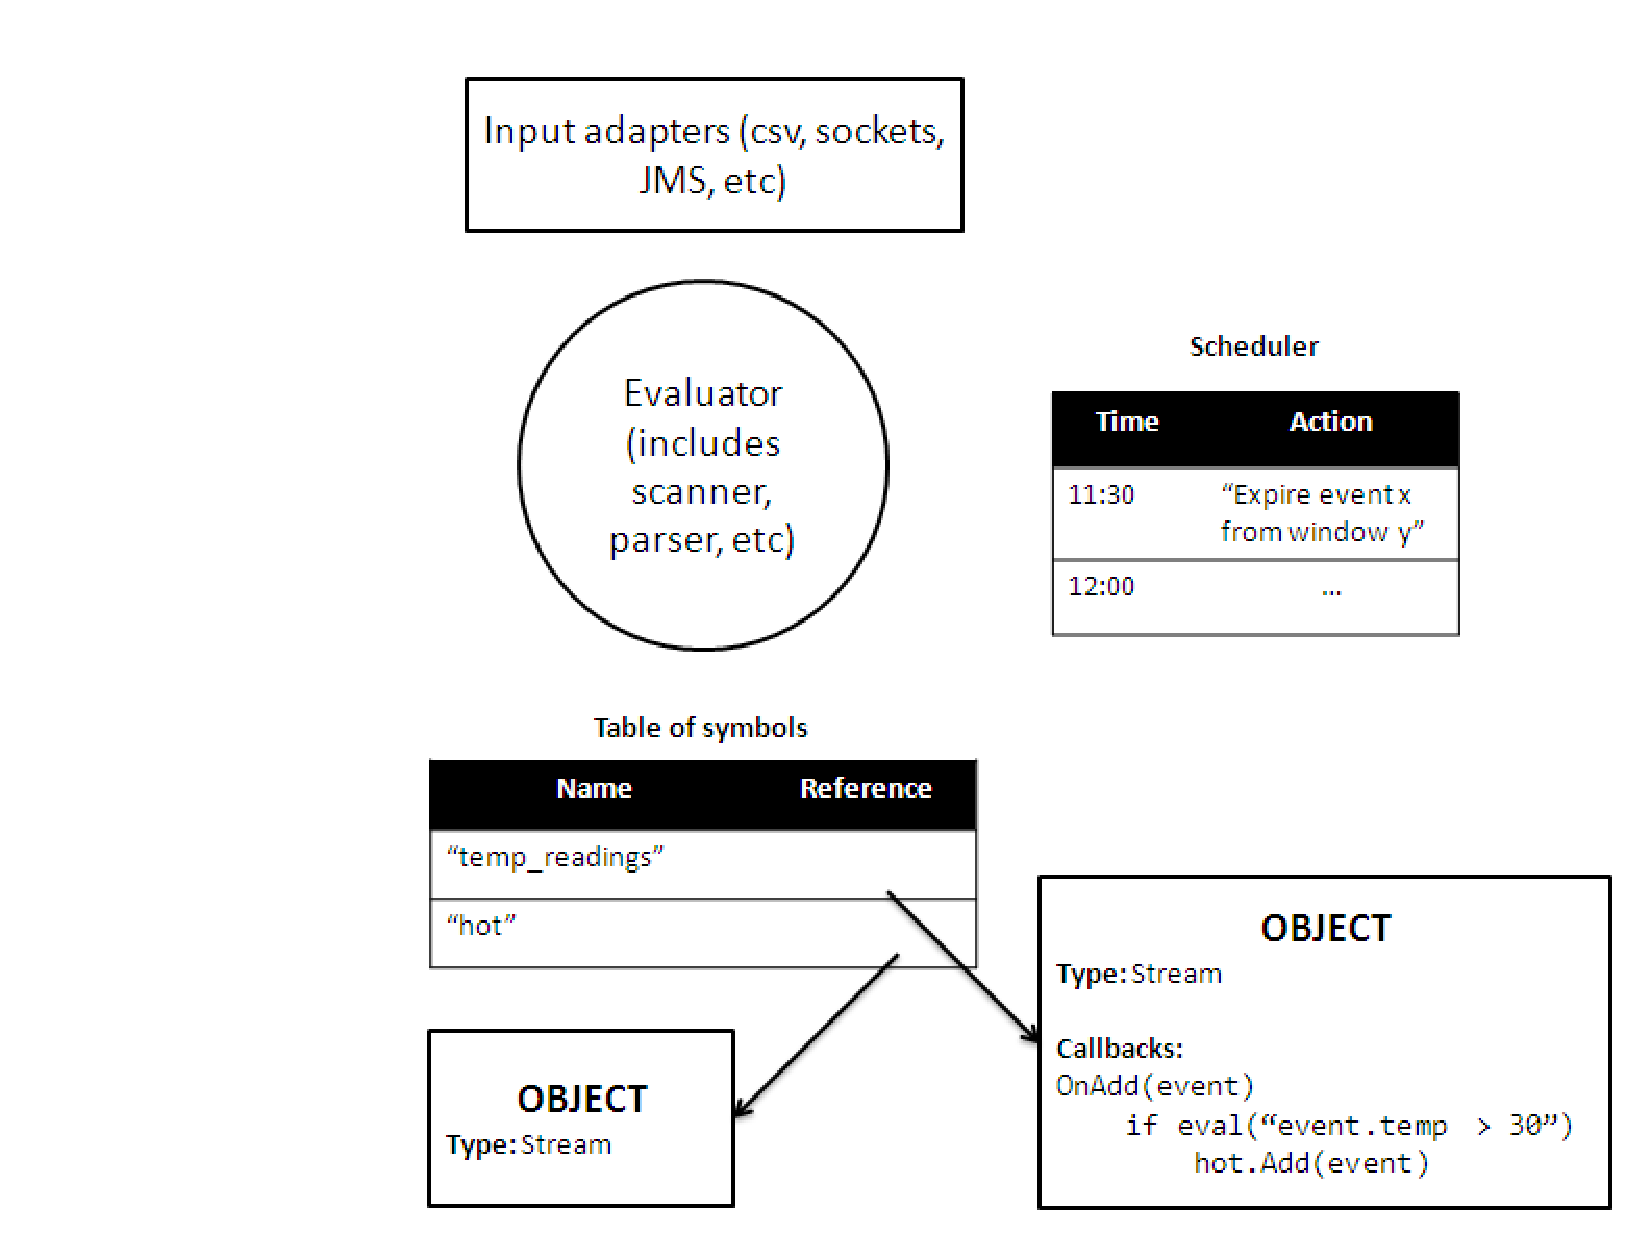
\includegraphics[width=\textwidth]{stupid_diagram}
  \caption{Major modules of the prototype}
\end{figure}


\section{Internal representation of values}

As mentioned above, objects are accessible through a table of
symbols. This subsection discusses how are objects represented
internally.

First of all, all values in this system are tagged with their
respective types. For example, the value \verb=123= will be tagged
with the type \verb=integer=. The same goes for streams, windows,
events, objects and everything else. For example, the value of
\verb=temp_readings= will include the tag \verb=stream=.

Events are represented internally as dictionaries. The event
attributes are kept in the dictionary keys and the event values are
stored as dictionary values. Events are immutable.

Streams are represented internally as simple collections that receive
events but do not keep them (we have windows for that). These
collections support the analogous operations that an EzQL Stream
supports -- \verb=Where=, \verb=Select=, \verb=Add=, etc. They also
support an \verb=OnAdd= operation where callbacks may be registered.

Windows are treated similarly to streams except their internal
representation supports two additional operations --
\verb=GetContents= and \verb=OnExpire=, whose names should be
self-explanatory.

Objects shall be represented just like events -- as dictionaries.


\chapter{A word about syntax}

In the examples I wrote in this document, I used a SQL like
syntax. However, I don't plan to support this syntax in early versions
of the interpreter. Instead, queries will be written using simple
method calls:

\begin{verbatim}
cheap_tolls = Segment.all.where(s -> s.toll < 10)
\end{verbatim}

Remember, \verb=s -> s.toll < 10= is our syntax for lambda
functions.

Supporting the SQL like syntax is easy, but it is something I'd prefer
to do only once, in the end, to avoid the need to change it every time
a new operator is added.

Besides, I prefer the method-call syntax :)

\end{document}
